\chapter{온도, 엔트로피와 에너지}

\lectureoverview{온도는 처음에 사람용 온도계 눈금을 미시적 에너지 단위로 환산하는 과정에서 등장한다. 이에 대응하여 열역학적 엔트로피를 무차원 통계적 엔트로피로 환산하고 나면, 평형은 하나의 매개변수로 표시되는 확률분포들의 족으로 기술된다. 미분 \(dE/dS\)로 온도를 정의할 수 있고, 열역학 제1법칙과 제2법칙은 온도 차이가 에너지 흐름의 방향을 정하는 이유를 보여 준다.}

\section{환산 인자와 사람의 단위}

물리학의 여러 상수는 환산 인자다. 빛의 속도는 거리를 시간으로 환산한다.
\begin{equation}
 t=\frac{x}{c}.
\end{equation}
거리와 시간을 서로 호환되는 단위로 측정한다면 \(c=1\)로 놓을 수 있다. 물리적 효과가 사라지는 것은 아니다. 두 종류의 측정값을 하나의 공통 척도로 나타냈을 뿐이다.

볼츠만 상수도 같은 성격을 지닌다. 사람의 척도에 맞춘 온도계로 읽은 온도를 에너지로 환산한다. \emph{사람의 척도에 맞춘}이라는 표현이 중요하다. 이런 단위는 거시적 기기로 구현하고 판독할 수 있기 때문에 선택한 것이지, 미시적 동역학이 특별히 선택한 단위이기 때문은 아니다.

섭씨 눈금은 표준 압력에서 물의 어는점과 끓는점 사이의 간격을 백 등분하여 정했다. 켈빈은 같은 크기의 눈금을 사용하지만 절대영도를 영점으로 삼는다. 다른 물질이나 다른 온도 간격, 또는 화씨 눈금을 선택해도 수치는 달라지지만 물리학은 달라지지 않는다.

\begin{classroomqa}
\audiencequestion{화씨 눈금도 이미 17세기에 만들어졌나요?}
\lecturerresponse{정확한 날짜는 여기서 중요하지 않다. 요점은 이런 눈금들이 모두 사람들이 만들고 측정할 수 있는 온도를 기준으로 고안되었다는 것이다. 눈금의 크기는 관례로 정한 것이지 미시적 기준에서 나온 것이 아니다.
\lecturetimestamp{00:01:34--00:01:50}}
\end{classroomqa}

이 눈금들이 만들어질 당시에는 열의 분자적 기원을 실험으로 밝힐 수 없었다. 거시적 온도계로 1도 변화를 관측할 수는 있었지만 분자 하나의 에너지는 측정할 수 없었다. 그러므로 온도가 근본적으로 에너지 척도라는 사실을 알기 전에 온도 단위를 정한 것은 자연스러운 일이었다.

\section{온도의 단위가 에너지인 이유}

희박 단원자 기체를 생각하자. 여기서 희박하다는 것은 현재 목적상 분자 사이의 상호작용 에너지를 무시할 수 있다는 뜻이다. 열평형에서는 등분배 법칙에 따라 각 이차 병진 자유도에 볼츠만 상수와 \(T_{\mathrm K}/2\)의 곱이 배정된다. 세 공간 차원에서는 \begin{equation}
 \left\langle E_{\mathrm{kin}}\right\rangle
 =\frac{3}{2}k_{\mathrm B}T_{\mathrm K}.
 \label{eq:sm2-equipartition-kelvin}
\end{equation} 인자 세는 \(x\), \(y\), \(z\) 방향의 운동을 센다. 절반이라는 계수는 이차 운동 에너지에서 비롯된다.

이 관계는 특정한 분자 종류에만 해당하지 않는다. 평형 상태의 헬륨과 산소 혼합물에서는 자유롭게 병진 운동하는 모든 입자의 질량중심 운동에너지가 평균적으로 같다. 무거운 입자가 더 느리게 움직이더라도 그렇다. 왜냐하면
\begin{equation}
 E_{\mathrm{kin}}=\frac{1}{2}mv^2,
\end{equation}
특징적인 에너지가 같으면 \(v\propto m^{-1/2}\)이기 때문이다.

같은 생각을 일부러 극단적인 사례에 적용해 볼 수도 있다. 볼링공을 유체에 담가 두고 계 전체가 평형에 이르게 하자. 볼링공의 브라운 병진 자유도도 분자의 자유도와 같은 에너지 척도로 결정된다. 볼링공의 속도는 질량이 엄청나게 크기 때문에 터무니없을 만큼 작지만, 온도는 속도가 아니라 에너지 척도를 비교한다.

실온에서 \(T_{\mathrm K}\)은 약 \(300\,\mathrm K\)인 반면, 미시적 자유도 하나의 에너지는 줄 단위로 보면 매우 작다. 따라서 환산 인자도 매우 작다.
\begin{equation}
 k_{\mathrm B}\simeq 1.38\times10^{-23}\,
 \mathrm{J\,K^{-1}}.
 \label{eq:sm2-boltzmann-value}
\end{equation}
그 크기와 아보가드로 수의 관계는 우연이 아니다.
\begin{equation}
 R=N_{\mathrm A}k_{\mathrm B}.
\end{equation}
기체 상수 \(R\)은 몰 단위의 양을 나타내고, \(k_{\mathrm B}\)은 그에 대응하는 미시적 구성 입자 하나당 척도를 나타낸다.

기본 공식에는 \(k_{\mathrm B}T_{\mathrm K}\)라는 조합이 거듭 나타난다. 따라서 다음과 같이 정의하면 더 간결하다.
\begin{equation}
 T\equiv k_{\mathrm B}T_{\mathrm K}.
 \label{eq:sm2-energy-temperature}
\end{equation}
이제부터 \(T\) 자체의 단위는 에너지이며, \eqref{eq:sm2-equipartition-kelvin}은 다음과 같이 된다.
\begin{equation}
 \left\langle E_{\mathrm{kin}}\right\rangle=\frac{3}{2}T.
 \label{eq:sm2-equipartition-natural}
\end{equation}
에너지를 줄로 측정하면 온도도 줄로 측정한다. 에너지를 전자볼트로 측정하면 온도도 전자볼트로 측정한다. 자연에 온도 단위라는 새로운 단위가 따로 있는 것은 아니다.

\section{엔트로피에 관한 두 가지 관례}

엔트로피에서도 같은 환산이 나타난다. 거시적 열역학은 열기관 분석에서 발전했다. 카르노가 결정적인 열기관 논리를 제시했고, 클라우지우스가 나중에 열역학적 엔트로피와 기호 \(S\)를 도입했다. 여기서 쓰는 표기법에서는 이 거시적 양을 \(S_{\mathrm C}\)라고 하자. 그 단위는 에너지를 온도계 온도로 나눈 것이며, 예를 들면 켈빈당 줄이다.

통계적 엔트로피는 무차원이다. 이산 확률분포의 경우,
\begin{equation}
 S=-\sum_i p_i\log p_i.
 \label{eq:sm2-statistical-entropy}
\end{equation}
자연로그를 쓰면 공정한 이진 선택의 엔트로피는 \(\log2\)이다. 밑이 2인 로그를 쓰면 같은 양을 1비트라고 부른다. 두 엔트로피 관례는 다음 관계로 연결된다.
\begin{equation}
 S=\frac{S_{\mathrm C}}{k_{\mathrm B}},
 \qquad
 S_{\mathrm C}=k_{\mathrm B}S.
 \label{eq:sm2-entropy-conversion}
\end{equation}
\(\mathrm{J\,K^{-1}}\) 단위로는 적당한 크기인 거시적 값이 매우 큰 무차원 엔트로피에 대응한다. 이는 엄청나게 많은 미시적 구성 입자에 정보가 분포한 양을 세기 때문이다.

식 \eqref{eq:sm2-energy-temperature}와
\eqref{eq:sm2-entropy-conversion}는 여기서 전반적으로 사용할 관례를 정한다.
\[
 [T]=[\text{energy}],
 \qquad
 [S]=1.
\]
이제 계산에 쓰는 식에서는 볼츠만 상수가 사라질 수 있다. \(T\)를 \(k_{\mathrm B}T_{\mathrm K}\)로, \(S\)를 \(S_{\mathrm C}/k_{\mathrm B}\)로 바꾸면 언제든 볼츠만 상수를 되살릴 수 있다.

\begin{classroomqa}
\audiencequestion{계수 \(3/2\)를 제외하면, 새로 정의한 온도는 줄 단위로 측정한 에너지인가요?}
\lecturerresponse{그렇다. 에너지 단위로 줄을 선택했다면 온도도 줄 단위다. 줄은 MKS 단위계의 \(\mathrm{kg\,m^2\,s^{-2}}\)이다. 대신 전자볼트나 다른 에너지 단위를 써도 된다. 그러면 온도는 같은 단위로 나타내야 한다. 계수 \(3/2\)는 이상기체 사례에 해당할 뿐, 온도의 정의에 들어가는 값은 아니다.
\lecturetimestamp{00:15:49--00:16:45}}
\end{classroomqa}

\begin{classroomqa}
\audiencequestion{칠판에서 온도를 켈빈으로 지정한다면 \(k_{\mathrm B}\)은 정해진 상수가 아닌가요?}
\lecturerresponse{온도와 에너지의 단위를 모두 지정하면 그 값은 정해진다. 켈빈을 화씨도로, 줄을 전자볼트로 바꾸면 수치는 달라진다. 이것이 바로 환산 인자의 단위 의존성이다.
\lecturetimestamp{00:16:46--00:18:33}}
\end{classroomqa}

\begin{classroomqa}
\audiencequestion{볼츠만 상수의 수치는 실험으로 결정하나요?}
\lecturerresponse{그렇다. 역사적으로 이 값을 구하려면 원자에 관한 미시적 정보와 원자의 수밀도가 필요했다. 볼츠만은 이런 양들이 정확히 알려지기 전에 분자 에너지와 온도의 관계를 이해했다. 이는 뉴턴이 중력 상수가 정확히 측정되기 전에 그 역할을 알았던 것과 비슷하다.
\lecturetimestamp{00:18:46--00:20:00}}
\end{classroomqa}

\section{평형은 통계적 상태다}

단위를 환산하는 것만으로는 아직 온도가 정의되지 않는다. 뜨거운 물체를 만지는 경험은 유용한 생물학적 직관을 주지만, 온도는 에너지와 엔트로피로부터 구성되는 유도 물리량이다.

거시적 조건이 고정된 큰 환경과 접촉한 계를 생각해 보자. 두 계 사이에 에너지가 오갈 수 있다. 계의 에너지가 처음에 지나치게 많으면 평균적으로 에너지를 잃고, 너무 적으면 평균적으로 얻는다. 열평형에서도 미시적 에너지 교환은 계속되지만 어느 쪽으로도 평균적인 순흐름은 없다.

\(i\)로 계의 정확한 미시 상태를 나타내고 그 상태의 에너지를 \(E_i\)로 쓰자. 평형이란 계가 한 상태에 고정된다는 뜻이 아니다. 환경과의 상호작용으로 미시 상태가 계속 바뀌므로, 각 가능한 상태에 확률 \(P_i\)를 부여한다. 기본 관계는 다음과 같다.
\begin{align}
 \sum_i P_i &=1,
 \label{eq:sm2-normalization}\\
 \sum_i P_iE_i &=\overline E,
 \label{eq:sm2-mean-energy}\\
 S&=-\sum_iP_i\log P_i.
 \label{eq:sm2-equilibrium-entropy}
\end{align}
\(\overline E\) 위의 가로줄은 부분계의 에너지가 요동한다는 점을 강조한다. 한 번 측정하면 한 값이 나오고 다음 측정에서는 다른 값이 나올 수 있다. 측정을 거듭하면 평균이 \eqref{eq:sm2-mean-energy}인 분포로 수렴한다.

\begin{figure}[t]
\centering
\includegraphics[width=0.82\textwidth]{lecture_02_figure_02.png}
\caption{칠판에 적힌 정규화와 평균 에너지:
\(\sum_iP(i)=1\) 및 \(\sum_iP(i)E(i)=\langle E\rangle\).}
\lectureframe{00:24:10}
\end{figure}

\section{평균 에너지로 표시되는 분포족}

평형 분포는 평균 에너지에 크게 좌우된다. 물 냄비를 난로 위에 올리면 \(\overline E\)가 높아지고, 눈 속에 두면 \(\overline E\)가 낮아진다. 확률도 이에 따라 변한다. 그러므로 평형은 하나의 분포가 아니라 매개변수 하나로 표시되는 분포족으로 보아야 한다.
\begin{equation}
 P_i(\overline E).
 \label{eq:sm2-family}
\end{equation}
각 분포는 다음 조건을 만족한다.
\begin{align}
 \sum_iP_i(\overline E)&=1,
 \label{eq:sm2-family-normalization}\\
 \sum_iP_i(\overline E)E_i&=\overline E.
 \label{eq:sm2-family-mean}
\end{align}

\begin{figure}[t]
\centering
\includegraphics[width=0.88\textwidth]{lecture_02_figure_03.png}
\caption{\(P(i,\overline E)\)로 넘어가는 장면이다. 분포족을 도입하는 동안 앞서 나온 정규화, 평균 에너지, 엔트로피 식은 계속 보이도록 둔다.}
\lectureframe{00:26:29}
\end{figure}

도식적인 그래프를 그릴 때는 \(E_i\)가 증가하는 순서대로 상태들을 배열한다. 그러면 가로축은 지표 \(i\) 또는 그에 대응하는 에너지로 읽을 수 있다. 평균 에너지가 높아질수록 확률 가중치는 더 오른쪽에 있는 상태들 쪽으로 이동한다. 모든 곡선은 전체 면적이 단위값을 유지해야 한다.

\begin{figure}[t]
\centering
\includegraphics[width=0.88\textwidth]{lecture_02_figure_04.png}
\caption{여러 개의 개략적 분포 \(P(i,\overline E)\). 확률이 더 오른쪽에 집중된 곡선일수록 평균 에너지가 크며, 모든 곡선은 정규화되어 있다.}
\lectureframe{00:28:40}
\end{figure}

\begin{figure}[t]
\centering
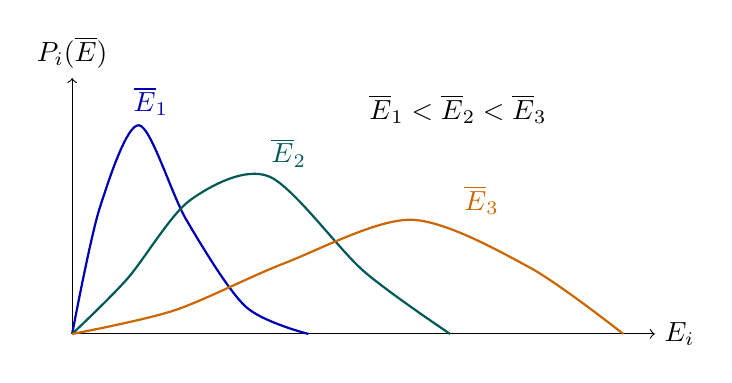
\begin{tikzpicture}[x=1cm,y=1cm]
\draw[->] (0,0) -- (7.4,0) node[right] {$E_i$};
\draw[->] (0,0) -- (0,3.25) node[above] {$P_i(\overline E)$};
\draw[thick,blue!70!black]
  plot[smooth] coordinates {(0,0) (0.35,1.6) (0.85,2.65) (1.45,1.45)
  (2.2,0.35) (3.0,0)};
\draw[thick,teal!70!black]
  plot[smooth] coordinates {(0,0) (0.7,0.7) (1.5,1.7) (2.5,2.0)
  (3.7,0.8) (4.8,0)};
\draw[thick,orange!80!black]
  plot[smooth] coordinates {(0,0) (1.3,0.3) (2.7,0.9) (4.3,1.45)
  (5.8,0.85) (7.0,0)};
\node[blue!70!black] at (1.0,2.95) {\(\overline E_1\)};
\node[teal!70!black] at (2.75,2.3) {\(\overline E_2\)};
\node[orange!80!black] at (5.2,1.7) {\(\overline E_3\)};
\node at (4.9,2.85) {\(\overline E_1<\overline E_2<\overline E_3\)};
\end{tikzpicture}
\caption{칠판 스케치를 깔끔하게 다시 그린 것이다. 곡선이 정확히 이런 모양일 필요는 없다. 여기서 사용하는 것은 정규화와 평균 에너지의 순서뿐이다.}
\end{figure}

\begin{classroomqa}
\audiencequestion{표기가 순환 논리가 아닌가요? 평균 에너지는 분포로 계산하는데, 분포는 평균 에너지로 표시하잖아요.}
\lecturerresponse{경험적으로 선택한 매개변수 하나짜리 평형 분포족에서 시작하자. 각 분포에는 평균 에너지가 있다. 분포마다 평균 에너지가 서로 다르다면 그 평균값을 분포족의 이름을 정하는 매개변수로 쓸 수 있다. 이 표기만으로 분포족이 유도되는 것은 아니다. 그 유도는 나중에 볼츠만 분포가 제시한다.
\lecturetimestamp{00:28:35--00:29:44}}
\end{classroomqa}

\begin{classroomqa}
\audiencequestion{왜 전체 에너지가 아니라 평균 에너지라고 하나요?}
\lecturerresponse{부분계는 열저장고와 에너지를 주고받는다. 예를 들어 기체 용기의 열이 통하는 벽 바깥에 있는 대기가 열저장고가 될 수 있다. 부분계의 순간 에너지는 요동한다. 여러 차례 측정하면 분포가 나오고 \(\overline E\)는 그 측정 결과들의 평균이다. 부분계와 열저장고를 합친 더 큰 닫힌 계의 에너지는 여전히 일정할 수 있다.
\lecturetimestamp{00:29:46--00:30:56}}
\end{classroomqa}

\begin{classroomqa}
\audiencequestion{서로 다른 미시 상태가 에너지는 같을 수 있나요? 서로 다른 분포의 평균 에너지도 같을 수 있나요?}
\lecturerresponse{둘 다 가능하다. 평균 에너지 제약만으로는 여러 분포가 허용되므로, 특별한 한 매개변수 평형 분포족을 정하려면 추가적인 물리적 논증이 필요하다. 그 기원과 볼츠만 분포의 형태는 나중에 유도할 것이다. 서로 다른 미시 상태가 같은 에너지를 갖는 문제는 축퇴라고 부르는 별개의 문제다.
\lecturetimestamp{00:30:58--00:32:22}}
\end{classroomqa}

\subsection{상태 표지, 축퇴, 상관관계}

혼동하기 쉬운 몇 가지 구분을 서로 분명히 나누어야 한다.

첫째, 평균 에너지가 같은 확률분포는 여러 개일 수 있다. 평균 에너지 제약만으로 한 매개변수 평형 분포족이 정해지는 것은 아니다. 그것은 평형화 과정에서 선택되는 특별한 분포족이며, 그 형태가 볼츠만 분포임을 나중에 확인할 것이다.

둘째, 서로 다른 미시 상태 여러 개가 같은 에너지를 가질 수 있다. 이를 축퇴라고 한다. 상태를 에너지 순서에 따라 모호함 없이 배열할 수 있도록, 칠판 설명에서는 정확히 같은 에너지를 갖는 경우를 잠시 무시한다. 대칭성이 있는 계에서는 축퇴가 흔하지만 개념적인 문제는 없다. 상태 표지 \(i\)를 유지하고, \(E_i\)가 같은 값을 가질 수 있도록 허용한 뒤 모든 상태에 대해 합하면 된다.

셋째, 상관관계는 축퇴와 같은 말이 아니다. 상관관계는 두 확률변수의 결합분포에 관한 것으로, 하나를 알았을 때 다른 변수의 확률이 달라지는지를 묻는다. 하나의 미시 상태 목록에서 서로 배타적인 표지인 \(i\)와 \(j\)는 그 자체로 상관관계를 계산할 두 확률변수가 아니다.

\begin{classroomqa}
\audiencequestion{이 구성에서는 서로 다른 \(i\) 상태들이 독립이라고 가정하나요? 그중 두 상태가 상관되어 있다면 어떻게 되나요?}
\lecturerresponse{상태 표지는 하나의 미시적 확률변수가 취할 수 있는 값 하나다. 독립성과 상관관계는 결합분포를 이루는 두 변수가 있어야 정의되므로, 이 목록에 있는 서로 다른 두 표지에는 그 용어를 직접 적용할 수 없다. 서로 다른 상태의 에너지가 같은지는 축퇴에 관한 문제다.
\lecturetimestamp{00:32:23--00:33:22}}
\end{classroomqa}

\begin{classroomqa}
\audiencequestion{서로 다른 두 상태의 에너지가 정확히 같으면 어떻게 되나요?}
\lecturerresponse{그것이 축퇴다. 지금 그래프에서는 단순화를 위해 어떤 두 에너지도 같지 않다고 가정하고, 상태를 에너지가 낮은 순서대로 배열한다. 뒤에 나올 확률 공식에는 이 가정이 필요하지 않다. 축퇴 상태도 각각 별도로 센다.
\lecturetimestamp{00:33:23--00:34:04}}
\end{classroomqa}

\begin{classroomqa}
\audiencequestion{상태 번호 \(i\)의 의미는 임의적인가요?}
\lecturerresponse{미시 상태 자체는 임의적이지 않다. 각각은 정확한 기술에 필요한 모든 위치, 운동량 또는 다른 데이터를 지정한다. 다만 상태의 이름은 임의적이므로 그림에서는 에너지가 증가하는 순서대로 번호를 붙인다.
\lecturetimestamp{00:34:06--00:35:15}}
\end{classroomqa}

\section{엔트로피는 에너지의 함수가 된다}

평형 분포족의 각 원소에는 엔트로피가 있다. \eqref{eq:sm2-family}를 \eqref{eq:sm2-equilibrium-entropy}에 대입하면 다음과 같다.
\begin{equation}
 S(\overline E)
 =-\sum_iP_i(\overline E)\log P_i(\overline E).
 \label{eq:sm2-entropy-energy}
\end{equation}
이는 모든 물리계에 공통인 하나의 함수가 아니다. 계의 에너지 준위 구조와 평형 분포족에 따라 달라진다. 그러나 그 분포족이 정해지면 에너지와 엔트로피가 연결된다. 분포족을 따라 변하면 두 양이 모두 변한다.

보통의 계에서는 평균 에너지가 커질수록 확률이 분포하는 상태 수가 늘어나므로, \(S\)는 대개 \(\overline E\)와 함께 증가한다. 일단 이 관계가 매끄럽고 국소적으로 역함수를 갖는다고 가정하자. 예외도 중요하지만, 단순한 경우를 보면 필요한 정의를 분명히 알 수 있다.

\section{온도를 정의하는 미분}

구체적으로 물어 보자. 엔트로피를 이진 선택 하나만큼 늘리려면 평균 에너지는 얼마나 변해야 하는가? 자연로그 단위에서 그 엔트로피 증가량은 \(\log2\)이다.

매끄러운 분포족에서 서로 가까운 두 원소에 대해,
\begin{equation}
 dE=\frac{dE}{dS}\,dS.
 \label{eq:sm2-differential-identity}
\end{equation}
이 단계에서 이 식은 그저 연쇄 법칙이다. 그러나 계수의 차원과 물리적 역할은 온도에 필요한 조건과 정확히 일치한다.

에너지 단위로 나타낸 온도는 다음과 같다.
\begin{definition}
\begin{equation}
 T\equiv\frac{dE}{dS}.
 \label{eq:sm2-temperature-definition}
\end{equation}
같은 뜻으로,
\begin{equation}
 dE=T\,dS,
 \qquad
 dS=\frac{1}{T}\,dE.
 \label{eq:sm2-fundamental-differentials}
\end{equation}
\end{definition}

1비트만큼 충분히 작게 변하는 경우,
\begin{equation}
 \Delta E\simeq T\log2.
 \label{eq:sm2-one-bit-energy}
\end{equation}
1비트에 주목하는 것은 미분의 의미를 구체적으로 드러내기 위한 방법일 뿐이다. 작은 엔트로피 변화라면 무엇이든 같은 국소 관계를 따른다.

\begin{classroomqa}
\audiencequestion{엔트로피를 \(S(E)\)로 썼다면, \(dS/dE\)가 더 자연스러운 미분 아닌가요?}
\lecturerresponse{관계가 국소적으로 역함수를 가지면 두 미분은 같은 정보를 담고 있다.
\[
 \frac{dE}{dS}=\left(\frac{dS}{dE}\right)^{-1}.
\]
관례상 온도는 \(dE/dS\)이고, 역온도는 \(dS/dE=1/T\)이다.
\lecturetimestamp{00:40:24--00:40:54}}
\end{classroomqa}

여기서는 열역학 변수가 하나만 변하므로 보통의 미분으로 충분하다. 부피, 입자 수, 자화 또는 다른 변수가 변할 수 있다면 편미분을 사용하고 어떤 양을 고정하는지 밝혀야 한다. 지금 정의한 온도는 더 일반적인 열역학적 기하에서 한 변수만 변하는 단면에 해당한다.

\subsection{볼츠만 상수가 소거되는 이유}

온도계 단위로 잠시 돌아가 보자. 다음을 사용하면
\[
 T=k_{\mathrm B}T_{\mathrm K},
 \qquad
 S=\frac{S_{\mathrm C}}{k_{\mathrm B}},
\]
기본 관계는 다음과 같이 된다.
\begin{align}
 dE
 &=\bigl(k_{\mathrm B}T_{\mathrm K}\bigr)
   d\left(\frac{S_{\mathrm C}}{k_{\mathrm B}}\right)\\
 &=T_{\mathrm K}\,dS_{\mathrm C}.
 \label{eq:sm2-carnot-form}
\end{align}
온도에서 \(k_{\mathrm B}\)가 한 번 곱해지고, 엔트로피에서는 그 역수가 곱해진다. 두 인자는 서로 소거된다. 이것이 보통의 열역학 교재에서 볼츠만 상수를 드러내지 않고 \eqref{eq:sm2-carnot-form}라고 쓸 수 있는 이유다.

\begin{classroomqa}
\audiencequestion{\(S(E)\)는 반드시 역함수를 가져야 하나요?}
\lecturerresponse{항상 그런 것은 아니다. 여기서 다루는 보통의 계에서는 에너지가 증가하면 평형 분포가 대체로 더 넓게 퍼지고 엔트로피도 증가한다. 따라서 \(S(E)\)는 단조 함수이고 \(T>0\)이다. 에너지 준위가 유계인 계는 반례가 될 수 있다. 여기에는 엔트로피가 에너지에 따라 감소하고 통계적 온도가 음수가 되는 영역도 포함된다. 그런 경우는 일단 여기서 다루지 않는다.
\lecturetimestamp{00:44:30--00:45:57}}
\end{classroomqa}

\section{추상적인 미분에서 뜨거움과 차가움으로}

미분으로 정의한 온도는 보편적이지만 아직 추상적이다. 뜨거운 물체에서 차가운 물체로 에너지가 흐른다는 익숙한 설명을 되찾고자 한다. 뜨거운 표면을 만질 때의 통증은 생물학적 현상이고, 색과 방출 복사는 빛의 성질에 좌우된다. 통계적 정의라면 복사를 무시한 이상화 기체에도 적용될 수 있어야 한다.

\begin{classroomqa}
\audiencequestion{뜨거운 물체가 내는 빛을 온도의 기본 정의에 이용할 수 있을까요?}
\lecturerresponse{복사는 유용한 온도계지만 빛의 물리학을 끌어들인다. 통계역학은 광학적 성질에 의존하지 않고 기체 상자 같은 계의 온도도 정의해야 한다. 에너지 교환의 방향이 더 일반적인 기준이다.
\lecturetimestamp{00:46:42--00:47:20}}
\end{classroomqa}

\(A\)와 \(B\) 두 계를 각각 처음에는 고유한 평형 상태에 두고, 온도를 각각 \(T_A\)와 \(T_B\)로 하자. 처음에는 두 계가 서로 고립되어 있다. 그런 다음 \emph{가느다란 관}을 통해 두 계를 약하게 열접촉시킨다. 이 관으로는 각 부분계의 정체성을 유지하면서 적은 양의 에너지가 오갈 수 있다.

\begin{figure}[t]
\centering
\includegraphics[width=0.88\textwidth]{lecture_02_figure_05.png}
\caption{온도 \(T_A\)와 \(T_B\)로 표시한 두 계 \(A\)와 \(B\)를 각각 따로 준비한 뒤, 약한 열접촉을 고려하기 직전의 모습.}
\lectureframe{00:48:55}
\end{figure}

\begin{figure}[t]
\centering
\begin{tikzpicture}[>=Stealth]
\draw[rounded corners,thick,fill=blue!6] (0,0) rectangle (2.6,2.4);
\draw[rounded corners,thick,fill=orange!8] (5.4,0) rectangle (8,2.4);
\draw[thick] (2.6,1.35) -- (5.4,1.35);
\draw[thick] (2.6,1.05) -- (5.4,1.05);
\draw[<->,very thick] (3.15,1.2) -- (4.85,1.2)
  node[midway,above] {\(\delta E\)};
\node at (1.3,1.45) {\Large \(A\)};
\node at (6.7,1.45) {\Large \(B\)};
\node at (1.3,0.65) {\(T_A,S_A,E_A\)};
\node at (6.7,0.65) {\(T_B,S_B,E_B\)};
\node at (4,0.35) {\small weak thermal contact};
\end{tikzpicture}
\caption{결합된 계는 고립된 채로 유지되고, 에너지는 약한 접촉을 통해 요동하며 오간다.}
\end{figure}

일반성을 잃지 않고 다음과 같이 가정하자.
\begin{equation}
 T_B>T_A.
 \label{eq:sm2-temperature-order}
\end{equation}
경험에 따르면 \(B\)는 에너지를 잃고 \(A\)는 에너지를 얻는다. 이 예상을 계산으로 확인하는 데는 세 가지 사실이 필요하다.

\subsection{엔트로피의 가법성}

미시적 선택지가 서로 독립적으로 결합하는 약결합 부분계 두 개에서는 결합된 경우의 수가 곱해진다.
\[
 W_{AB}=W_AW_B.
\]
엔트로피는 로그 함수이므로,
\begin{equation}
 S_{\mathrm{tot}}=S_A+S_B.
 \label{eq:sm2-entropy-additivity}
\end{equation}
곱 분포의 섀넌 엔트로피에서 직접 출발해도 같은 결과를 얻는다.

\begin{classroomqa}
\classquestion{결합된 계의 엔트로피가 왜 더해지나요?}
\lecturerresponse{바탕이 되는 선택지의 수는 곱해지고 엔트로피는 로그를 취하기 때문이다.
\(\log(W_AW_B)=\log W_A+\log W_B\). 약한 상호작용이 있어야 부분계로 기술할 수 있고, 이 선도 차수의 가법성이 성립한다.
\lecturetimestamp{00:51:06--00:52:03}}
\end{classroomqa}

\subsection{열역학 제1법칙과 제2법칙}

결합된 계는 고립되어 있으므로 내부에서 교환되는 에너지는 보존된다.
\begin{equation}
 dE_A+dE_B=0,
 \qquad
 dE_B=-dE_A.
 \label{eq:sm2-first-law}
\end{equation}
이 실험에서 이것이 열역학 제1법칙이다.

열역학 제2법칙은 여기서 가정으로 삼고, 그 더 깊은 설명은 나중으로 미룬다. 접촉한 계들이 새로운 평형으로 이완할 때,
\begin{equation}
 dS_{\mathrm{tot}}=dS_A+dS_B\geq0.
 \label{eq:sm2-second-law}
\end{equation}
엄격한 부등식은 평형에서 벗어나 자발적으로 이완하는 과정을 나타낸다. 가역적인 1차 변분으로 평형 상태에 있을 때는 등호가 성립한다.

마지막으로 온도의 정의를 각 부분계에 적용하면 다음과 같다.
\begin{equation}
 dE_A=T_A\,dS_A,
 \qquad
 dE_B=T_B\,dS_B.
 \label{eq:sm2-two-temperatures}
\end{equation}

\begin{figure}[H]
\centering
\includegraphics[width=0.88\textwidth]{lecture_02_figure_06.png}
\caption{칠판 논증의 끝에 나온 두 부분계의 관계
\(dE_A=T_A\,dS_A\) 및 \(dE_B=T_B\,dS_B\).}
\lectureframe{00:54:00}
\end{figure}

\subsection{에너지 흐름의 방향}

이 식들만으로도 순에너지 이동의 방향이 정해진다. \(dS_A=dE_A/T_A\), \(dS_B=dE_B/T_B\) 및
\eqref{eq:sm2-first-law}를 \eqref{eq:sm2-second-law}에 대입하자.
\begin{align}
 dS_{\mathrm{tot}}
 &=\frac{dE_A}{T_A}+\frac{dE_B}{T_B}\\
 &=dE_A\left(\frac{1}{T_A}-\frac{1}{T_B}\right)\geq0.
 \label{eq:sm2-flow-sign}
\end{align}
\(T_B>T_A>0\)라면,
\[
 \frac{1}{T_A}-\frac{1}{T_B}>0.
\]
따라서 식 \eqref{eq:sm2-flow-sign}는 다음을 요구한다.
\[
 dE_A>0,
 \qquad
 dE_B<0.
\]
더 차가운 계 \(A\)는 에너지를 얻고 더 뜨거운 계 \(B\)는 에너지를 잃는다. \(T_A=T_B\)일 때는 엔트로피의 1차 변화가 선호되는 방향을 정하지 않으며, 미시적 교환은 균형을 이루어 순흐름이 0이 된다. 이처럼 추상적인 미분 \(T=dE/dS\)은 뜨거움과 차가움의 조작적 구분을 재현한다.
